%   ####
%
%   Band VIII, 3 N.~??A12
%   Signatur/Tex-Datei: LH_35_09_15_018-019
%   RK-Nr. 60649 (= ex 41154 A; ursprüngliche Zuschreibung korrigiert: RK 41154 und 41155 gehören nicht zusammen)
%   Überschrift: [De viribus chordas ad rupturam tendentibus (ex: De viribus chordas tendentibus)]
%   Datierung: [??August 1682 -- Sommer 1684??]
%   WZ: Gegenmarke G D (= RK-WZ: 273)
%.  SZ: (keins)
%.  Bilddateien (PDF): LH_35_09_15_018-019_d1; LH_35_09_15_018-019_d2; LH_35_09_15_018-019_d3; LH_35_09_15_018-019_d4 (insgesamt vier)
%
%
\begin{ledgroupsized}[r]{120mm}
\footnotesize
\pstart
\noindent\textbf{Überlieferung:}
\pend
\end{ledgroupsized}
\begin{ledgroupsized}[r]{114mm}
\footnotesize
\pstart \parindent -6mm
\makebox[6mm][l]{\textit{L}}%
Aufzeichnung: LH~XXXV~9,~15 Bl.~18\textendash19.
Ein Bogen~4\textsuperscript{o};
ein Wasserzeichen auf Bl.~19: Papier aus dem Harz.
Drei voll beschriebene Seiten.
Bl.~19~v\textsuperscript{o} ist leer.
% Zahlreiche Streichungen, Ergänzungen und Ersetzungen.
% Das Diagramm \lbrack\textit{Fig.~2}\rbrack\ auf Bl.~18~v\textsuperscript{o} ist zweifach ausgeführt.
\pend
\end{ledgroupsized}
%
%
\vspace{5mm}
\begin{ledgroup}
\footnotesize
\pstart
\noindent\footnotesize{%
%\textbf{Datierungsgründe:}
%Im Mittelpunkt der titellosen Aufzeichnung N.~??A12 steht das Verhältnis zwischen Ton\-hö\-he, Spannung und Dehnung elastischer Saiten, insbesondere mit Blick auf die Frage, bei welcher Spannung eine Saite reißt.
%Die Untersuchung geht u.a. von der Annahme aus, dass die Dehnung einer Saite in direk\-tem Verhältnis zur Spannung stehe \textendash\ eine Annahme, die Leibniz als \glqq bewiesen\grqq\ bezeichnet (S.~\refpassage{LH_35_09_15_018r_alias_sjhvbis-1}{LH_35_09_15_018r_alias_sjhvbis-2}; \refpassage{LH_35_09_15_019r_alibi_iocslg-1}{LH_35_09_15_019r_alibi_iocslg-2}).
%Damit spielt er höchstwahrscheinlich auf die Beweisführung an, die in % anderen Texten angeführt hat:
%den Aufzeichnungen N.~??A23, N.~??A20 und LH~XXXVII~3 Bl.~125\textendash127 sowie in einem Brief an E.~Mariotte vom März/April 1683 mit unterschiedlicher Ausführlichkeit dargelegt ist:
%An den Spannungszuständen einer Luftmasse in einem dichten Behälter lasse sich % unter Annahme der Aequipollenz von Ursache und Wirkung 
%allgemein zeigen, dass elastische Körper \textendash\ wie etwa Saiten \textendash\ sich in direktem Verhältnis zu ihren Spannkräften dehnen würden
%(siehe % N.~??A23, S.~\refpassage{LH_35_09_16_020v_kolbenmodell-1}{LH_35_09_16_020v_kolbenmodell-2}; N.~??A20, S.~\refpassage{LH_35_09_16_002_Beweis-1}{LH_35_09_16_002_Beweis-2}; LH~XXXVII~3 Bl.~125\textendash127; und den Brief an E.~Mariotte vom März/April 1683, \cite{01262}\textit{LSB} III,~3 N.~456, S.~795.21\textendash796.3
%für die einzelnen Nach\-wei\-se die Erläuterung zu S.~\refpassage{LH_35_09_15_018r_alias_sjhvbis-1}{LH_35_09_15_018r_alias_sjhvbis-2}).%
%\protect\index{Namensregister}{\textso{Mariotte}, Edme, Seigneur de Chazeuil ca. 1620\textendash1684}
%Auch die Aufzeichnung N.~??A07 knüpft eingangs (S.~\refpassage{LH_37_01_022r_grundhypothese_ihutd-1}{LH_37_01_022r_grundhypothese_ihutd-2}) an denselben \glqq Beweis\grqq\ an.
%Folglich kann N.~??A12 nicht vor den benannten, insgesamt auf die Zeitspanne zwischen ??August 1682 und der ersten Hälfte 1684?? datierbaren Texten verfasst worden sein.
%Der Terminus ante quem der Datierung entnimmt man dem im Texträger von N.??A12 vorliegenden Wasserzeichen, welches von einer Papiermühle aus dem Harz stammt und im Leibniz-Nachlass nach heutigem Kenntnisstand nur für den Zeit\-raum vom Dezember 1682 bis zum Sommer 1684 belegt ist (bei einem einzigen auf das Jahr 1686 datierten Vorkommnis der Gegenmarke ist fraglich, ob es sich um genau das gleiche Wasserzeichen handelt).
%Daraus ergibt sich die vorgeschlagene Datierung.
\textbf{Datierungsgründe:}\label{LH_35_09_15_018-019_Datierung}
Ausgangspunkt der titellosen Aufzeichnung N.~17 ist das Verhältnis zwischen Frequenz, Spannung und Dehnung schwingender Saiten oder Seile,
woraus sich dann die Frage ergibt, bei welcher Spannung eine Saite bzw. ein Seil reißt.
Die anschließende Untersuchung geht u.a. von der Annah\-me aus, dass die Dehnung einer Saite bzw. eines Seils in direktem Verhältnis zur Spannkraft stehe: eine Annahme, die Leibniz als \glqq bewiesen\grqq\ bezeichnet (S.~\refpassage{LH_35_09_15_018r_alias_sjhvbis-1}{LH_35_09_15_018r_alias_sjhvbis-2}; \refpassage{LH_35_09_15_019r_alibi_iocslg-1}{LH_35_09_15_019r_alibi_iocslg-2}).
Hierbei spielt er wahrscheinlich auf eine Beweisführung an, die im Kern bereits in der Aufzeichnung N.~7 (S.~\refpassage{LH_35_09_15_022v_Beweis_sgtk-1}{LH_35_09_15_022v_Beweis_sgtk-2}) vorliegt, mit größerer Ausführlichkeit aber in den Entwürfen N.~14\textsubscript{3}, N.~14\textsubscript{7} und LH~XXXVII~3 Bl.~125\textendash127 sowie in Leibnizens Brief an E.~Mariotte von März/April 1683 dargelegt wird:
An den Spannungszuständen einer Luftmasse in einem verschlossenen Behälter lasse sich allgemein zeigen, wie sich Spannkraft und Dehnung bei elastischen Körpern \textendash\ u.a. auch Saiten oder Seilen \textendash\ zueinander verhalten
(siehe für die Einzelnachweise die Erläuterung zu S.~\refpassage{LH_35_09_15_018r_alias_sjhvbis-1}{LH_35_09_15_018r_alias_sjhvbis-2}).%
\protect\index{Namensregister}{\textso{Mariotte}, Edme, Seigneur de Chazeuil ca. 1620\textendash1684}
Folglich dürfte N.~17 nicht vor den genannten Texten verfasst worden sein.
Die Aufzeichnung N.~7 ist auf die Zeitspanne zwischen Sommer 1678 und Winter 1680/1681 datierbar (siehe die Begründung, S.~\pageref{LH_35_09_15_001,022_Datierung});
die mit dem genannten Brief an Mariotte eng verbundenen Entwürfe N.~14\textsubscript{3} und N.~14\textsubscript{7} entstanden insgesamt zwischen Ende Januar 1683 und der ersten Hälfte 1684 (siehe die editorische Vorbemerkung zum Textkomplex N.~14, S.~\refpassage{AE_1684_319-325_intro_LeibizAnMariotte-1}{AE_1684_319-325_intro_LeibizAnMariotte-1}\,ff.);\protect\index{Namensregister}{\textso{Mariotte}, Edme, Seigneur de Chazeuil ca. 1620\textendash1684}
die Entstehungszeit des Entwurfs LH~XXXVII~3 Bl.~125\textendash127 ist noch nicht ermittelt (dieser Text wird voraussichtlich in einem künftigen Band von \textit{LSB} VIII ediert). 
Als besonders datierungsrelevant erweist sich allerdings die inhaltliche Aus\-richtung der mit grundlegenden Themen der Elastizität und Festigkeit befassten Entwürfe N.~14\textsubscript{3} und N.~14\textsubscript{7}:
Diese räumen, ihrem thematischen Ansatz gemäß, der (für N.~17 zentralen) Frage, unter welchen Bedingungen gespannte Körper reißen, eine grundlegende Bedeutung ein, weshalb N.~17 gleichsam als Ableger der Ausführungen in N.~14\textsubscript{3} und N.~14\textsubscript{7} angesehen werden kann.
Eine frühere Entstehungszeit der Aufzeichnung N.~17 ist somit unwahrscheinlich.
}%
\pend%
\pstart%
\footnotesize{
Weitere datierungsrelevante Informationen liefert das im Textträger von N.~17 vorliegende Wasserzeichen, das von einer Papiermühle aus Osterode stammt und im Leibniz-Nachlass nach heutigem Kenntnisstand lediglich für den Zeitraum 1683 bis 1684 belegt ist (bei einem einzigen auf das Jahr 1686 datierten Vorkommnis der Gegenmarke ist fraglich, ob es sich überhaupt um das gleiche Wasserzeichen handelt).%
\protect\index{Ortsregister}{Osterode}%
\protect\index{Ortsregister}{Harz}
Das identifizierte Papier bestätigt somit den Terminus post quem der Datierung von N.~17 und liefert zugleich einen glaubwürdigen Terminus ante quem.
Daraus ergibt sich, dass die vorliegende Aufzeichnung wahrscheinlich im Zeitraum von Ende Januar 1683 bis zum Ende des Jahres 1684 entstand.
% (1) Gleiches Wasserzeichen wie im Stück N.~??A04.2, Blatt 4 und Blatt 6: C D (RK-WZ: 273).\\
% (2) Inhaltlicher Zusammenhang mit N.~???    (3) ??????    (4) ??????
}%
\pend
\end{ledgroup}
\newpage
% \vspace{1.5em}%
 %  \newpage
%  \edtext{}{\lemma{\lbrack\textit{Fig.~1}\rbrack}\killnumber\Cfootnote{**************************}}
%  \newpage
  %\vspace*{1.0em}%
%%
%
%
%\vspace{4mm}
\count\Bfootins=900
\count\Afootins=900
\count\Cfootins=900
\pstart%
\normalsize%
\noindent%
%
\lbrack18~r\textsuperscript{o}\rbrack\ % % % % Blatt 18r
%
% \pend%
% Überschrift
% \pstart%
% \centering%
% ****
% \pend%
% \vspace*{1.0em}%
%
% \pstart%
% \noindent%
Tonos chordarum\protect\index{Sachverzeichnis}{tonus chordae}
esse in subduplicata ratione virium
\edtext{tendentium,\protect\index{Sachverzeichnis}{vis tendens}
\edtext{alibi}{%
\lemma{alibi}\Cfootnote{%
In N.~8\textsubscript{4} findet sich ein derartiger Beweis tatsächlich (S.~\refpassage{LH_35_09_15_012r_utsubduplrt-3}{LH_35_09_15_012r_utsubduplrt-5}); er wird aber so\-gleich widerlegt (S.~\refpassage{LH_35_09_15_013r_widerlegung-1}{LH_35_09_15_013r_widerlegung-2}).}}%
}{%
\lemma{tendentium,}\Bfootnote{%
\hspace*{-0,5mm}\textbar~seu si ita appellare placet, tensionum, \textit{gestr.}~%
\textbar\ alibi%
~\textit{L}}}
\edtext{demonstratum est.
Et rursus
\edtext{\edlabel{LH_35_09_15_018r_alias_sjhvbis-1}alias\edlabel{LH_35_09_15_018r_alias_sjhvbis-2}}{%
\lemma{alias}\Cfootnote{%
Siehe zu diesem \glqq Beweis\grqq\ die Entwürfe N.~14\textsubscript{3} (S.~\refpassage{LH_35_09_16_020v_kolbenmodell-1}{LH_35_09_16_020v_kolbenmodell-2}), N.~14\textsubscript{7} (S.~\refpassage{LH_35_09_16_002_Beweis-1}{LH_35_09_16_002_Beweis-2}) und LH~XXXVII~3 Bl.~125\textendash127 (in einem späteren Band der Reihe VIII) sowie Leibnizens Brief an E.~Mariotte vom März/April 1683 (\cite{01262}\textit{LSB} III,~3 N.~456, S.~795.21\textendash796.3).}}
demostratum est,
ejusdem chordae diversarum longitudinum\protect\index{Sachverzeichnis}{longitudo chordae}
differentias esse ut vires tendentes.}{%
\lemma{demonstratum}\Bfootnote{%
\hspace*{-0,5mm}est
\textit{(1)}~, eaedem autem sunt in ratione simplici longitudinum. Ergo longitudines
\textit{(2)}~. Et rursus \lbrack...\rbrack\ ejusdem chordae
\textit{(a)}~tensiones diversas
\textit{(b)}~diversarum longitudinum \lbrack...\rbrack\ vires tendentes.%
~\textit{L}}}
At si eadem manente tensione\protect\index{Sachverzeichnis}{tensio chordae}
diversae partes accipiantur,
erunt vires tendentes in duplicata ratione
\edtext{partium;
quia}{%
\lemma{partium}\Bfootnote{%
\textit{(1)}~. Hinc sequitur
\textit{(2)}~; quia%
~\textit{L}}}
toni earum sunt ut
\edtext{longitudines,\protect\index{Sachverzeichnis}{longitudo chordae}
vires autem}{%
\lemma{longitudines,}\Bfootnote{%
\textit{(1)}~vires au
\textit{(2)}~toni
\textit{(3)}~vires autem%
~\textit{L}}}
tendentes\protect\index{Sachverzeichnis}{vis tendens}
initio duximus esse in duplicata ratione tonorum.\protect\index{Sachverzeichnis}{tonus chordae}
\pend%
\pstart%
Chorda magis tensa\protect\index{Sachverzeichnis}{chorda tensa} facilius
\edtext{rumpitur
et quanta est vis tendens\protect\index{Sachverzeichnis}{vis tendens} chordam
tantum decedit potentiae ad rumpendum necessariae.%
\protect\index{Sachverzeichnis}{potentia ad rumpendum necessaria}
Sit pondus ad chordam non tensam rumpendam\protect\index{Sachverzeichnis}{pondus ad rumpendum necessarium}
necessarium \textit{p}.
Et sit chordae uno modo tensae vis tendens \textit{t},
sed magis adhuc tensae vis tendens sit $\theta.$\protect\index{Sachverzeichnis}{vis tendens}
Erit vis ad priore modo rumpendam\protect\index{Sachverzeichnis}{vis ad rumpendum necessaria}
necessaria}{%
\lemma{rumpitur}\Bfootnote{%
\textit{(1)}~. Magis tensa autem intelligitur in
\textit{(2)}~. Sit
\textit{(3)}~et quanta est vis tendens chordam
\textit{(a)}~tanto n
\textit{(b)}~tantum decedit \lbrack...\rbrack\ rumpendum necessariae.%
\textit{(aa)}~Si duae chordae ejusdem sint tensionis inaequalisque longitudinis,
id quod potentiae ad rumpendum necessariae decedit in
\textit{(bb)}~Sit pondus \lbrack...\rbrack\ necessarium \textit{p}
\textit{(aaa)}~erit
\textit{(bbb)}~et sit una Chordae
\textit{(aaaa)}~tend
\textit{(bbbb)}~vis tendens \textit{t}, altera $\theta,$ erit vis ad rumpendam chordam
\textit{(ccc)}~. Et sit chordae
\textit{(aaaa)}~una
\textit{(aaaaa)}~tensio \textit{t},
\textit{(bbbbb)}~vis
\textit{(bbbb)}~uno modo tensae vis tendens \textit{t},
\textit{(aaaaa)}~altero modo eadem sit $\theta$
\textit{(bbbbb)}~sed magis \lbrack...\rbrack\ sit $\theta.$
\textit{(aaaaa-a)}~Erit
\textit{(bbbbb-b)}~Erit vis ad
\textit{(aaaaa-aa)}~prioris
\textit{(bbbbb-bb)}~priorem
\textit{(ccccc-cc)}~priore modo rumpendam necessaria%
~\textit{L}}}
$p - t,$
sed ad posteriore modo tensam\protect\index{Sachverzeichnis}{chorda tensa}
rumpendam requiretur $p - \theta.$
Eritque earum differentia $\theta -
\edtext{\lbrack t\rbrack.}{\lemma{\textit{p}}\Bfootnote{\textit{L~ändert Hrsg.}}}$
Ergo differentia virium ad rumpendum\protect\index{Sachverzeichnis}{vis ad rumpendum necessaria}
necessariarum
\edtext{in eadem chorda}{%
\lemma{in}\Bfootnote{%
\hspace*{-0,5mm}eadem chorda \textit{erg.~L}}}
eadem est,
quae virium\protect\index{Sachverzeichnis}{vis tendens}
tendentium.\edlabel{LH_35_09_15_018r_piirros-1}
\edtext{}{{\xxref{LH_35_09_15_018r_piirros-1}{LH_35_09_15_018r_piirros-2}}{%
\lemma{tendentium.}\Bfootnote{%
\textit{(1)}~Hinc si chor
\textit{(2)}~Si
\textit{(a)}~tres
\textit{(b)}~plures sint chordae%
~\textit{L}}}}
\pend%
\vspace{1.5em}%
  \centerline{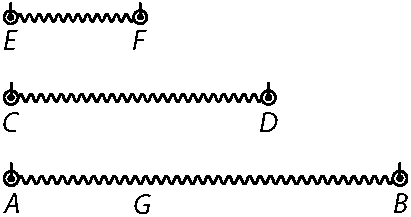
\includegraphics[width=0.36\textwidth]{gesamttex/edit_VIII,3/images/LH_35_09_15_018-019_d1.pdf}}%
  \vspace{0.5em}
  \centerline{\lbrack\textit{Fig.~1}\rbrack}%
      \newpage
%
\count\Bfootins=1000
\count\Afootins=1000
\count\Cfootins=1000
\pstart%
Si plures sint chordae\edlabel{LH_35_09_15_018r_piirros-2}\protect\index{Sachverzeichnis}{chorda tensa}
ejusdem
\edtext{crassitiei,\protect\index{Sachverzeichnis}{crassities chordae}
consistentiae\protect\index{Sachverzeichnis}{consistentia chordae}
et toni,\protect\index{Sachverzeichnis}{tonus chordae}}{%
\lemma{crassitiei}\Bfootnote{%
\textit{(1)}~et
\textit{(2)}~,~consistentiae et
\textit{(a)}~so
\textit{(b)}~toni%
~\textit{L}}}
longitudines\protect\index{Sachverzeichnis}{longitudo chordae}
autem sint progressionis arithmeticae,\protect\index{Sachverzeichnis}{progressio arithmetica}
ut \edtext{numeri ordine}{%
\lemma{numeri}\Bfootnote{%
% \hspace*{-0,5mm}
\textbar~in \textit{gestr.}~\textbar\ ordine%
~\textit{L}}}
naturali\protect\index{Sachverzeichnis}{ordo numerorum naturalis} sumti,
\edtext{erunt differentiae virium}{%
\lemma{erunt}\Bfootnote{%
\textit{(1)}~vires
\textit{(2)}~differentiae virium%
~\textit{L}}}
ad rumpendum necessariarum\protect\index{Sachverzeichnis}{vis ad rumpendum necessaria}
ut numeri impares.\protect\index{Sachverzeichnis}{numerus imparis}
Sit enim \textit{EF}, 1. et \textit{CD}, 2. et \textit{AB}, 3.
Erunt vires tendentes\protect\index{Sachverzeichnis}{vis tendens} ut 1. 4. 9.
Differentiae vero virium tendentium eaedem
quae ad rumpendum necessariarum,\protect\index{Sachverzeichnis}{vis ad rumpendum necessaria}
erunt 3. 5.
Si essent \textit{EF}, 3. et \textit{CD}, 4. et \textit{AB}, 5.
forent differentiae virium rumpentium\protect\index{Sachverzeichnis}{vis rumpens}
\edtext{7. 9.
\newline%
\indent%
Si\edlabel{LH_35_09_15_018r_aequtens-1}}{%
\lemma{7.~9.}\Bfootnote{%
\hspace*{-0,5mm}\textbar~Ex iis observationibus\protect\index{Sachverzeichnis}{observatio}
sequitur consideratio practica\protect\index{Sachverzeichnis}{consideratio practica}
magni momenti, nimirum laminis,\protect\index{Sachverzeichnis}{lamina}
vel tabulis\protect\index{Sachverzeichnis}{tabula} vel funibus\protect\index{Sachverzeichnis}{funis}
\textbar~ad resistendum ictui\protect\index{Sachverzeichnis}{ictus} \textit{erg.}~%
\textbar\ utendum esse longis et latis potius quam crassis,
quanto enim longior erit manente eadem, vel etiam existente minore tensione,\protect\index{Sachverzeichnis}{tensio}
eo minus facile rumpetur corpus Elasticum.\protect\index{Sachverzeichnis}{corpus elasticum}
\textit{gestr.}~\textbar\ Si%
~\textit{L}}}
duae chordae\protect\index{Sachverzeichnis}{chorda tensa}
sola longitudine differant,
vires tendentes\protect\index{Sachverzeichnis}{vis tendens}
sunt ut longitudines;\protect\index{Sachverzeichnis}{longitudo chordae}
\edtext{seu ad chordae \textit{AB} partem \textit{AG}
in hac tensione\protect\index{Sachverzeichnis}{tensio chordae}}{%
\lemma{seu}\Bfootnote{%
\textit{(1)}~chordae
\textit{(2)}~ad
\textit{(a)}~chordam \textit{AG} in praesenti
\textit{(b)}~chordae \textit{AB} partem \textit{AG} in hac
\textbar~eadem \textit{gestr.}~%
\textbar\ tensione%
~\textit{L}}}
conservandam opus est tantum pondere\protect\index{Sachverzeichnis}{pondus tendens}
quod sit ad pondus tendens chordam \textit{AB},
ut \textit{AG} ad \textit{AB}.
Perinde enim est ac si chorda divisa ponatur in partes aequales,
unaquaeque eodem pondere\protect\index{Sachverzeichnis}{pondus tendens}
in eadem tensione\protect\index{Sachverzeichnis}{tensio chordae} conservabitur,
cum discrimen sit nullum.\edlabel{LH_35_09_15_018r_aequtens-2}
Eadem autem vi opus
\edtext{est sive si}{%
\lemma{est}\Bfootnote{%
\hspace*{-0,5mm}sive
\textit{(1)}~ut
\textit{(2)}~si%
~\textit{L}}}
separatim pectentur,
sive in unum conjungantur.
Et pone unam manere,
vim autem quandam in iis pendulam eas tensas servare,
seu vim\protect\index{Sachverzeichnis}{vis tendens}
facere pati partem chordae,
ut si in \textit{G} pendeat verticillus,\protect\index{Sachverzeichnis}{verticillus}
quem ego vertam.
%
\lbrack18~v\textsuperscript{o}\rbrack\ % % % % Blatt 18v
%
Utique simul tam \edtext{partem \textit{AG},}{%
\lemma{partem}\Bfootnote{%
\textit{(1)}~\textit{AB}, 
\textit{(2)}~\textit{AG},%
~\textit{L}}}
 quam \textit{GB} tendam,
nec potest aliud cogitari quam vires
fore ut longitudines,\protect\index{Sachverzeichnis}{longitudo chordae}
certe si aequales sunt \textit{AG} et \textit{GB},
vires\protect\index{Sachverzeichnis}{vis tendens} erunt aequales.
Unde subdividendo rursus in partes
novisque adhibitis verticillis\protect\index{Sachverzeichnis}{verticillus}
manebit semper
\edtext{aequalitas. Pone enim}{%
\lemma{aequalitas.}\Bfootnote{%
\textit{(1)}~Possumus eni
\textit{(2)}~Pone enim%
~\textit{L}}}
in \textit{G} esse verticillum,\protect\index{Sachverzeichnis}{verticillus}
et \textit{AG} et \textit{GB} esse aequales\lbrack,\rbrack\
utique dimidia vis impendetur in \textit{AG},
altera dimidia in \textit{GB},
jam pone separari,
utique vis quae tetendit\protect\index{Sachverzeichnis}{vis tendens} \textit{GB},
sufficiet ad conservandam in tensione\protect\index{Sachverzeichnis}{tensio chordae} \textit{GB,}
nempe dimidia.
Chordam\protect\index{Sachverzeichnis}{chorda tensa} \textit{GB} similiter poterimus subdividere;
et ita dimidia ejus erit quarta
\edtext{\lbrack pars\rbrack}{\lemma{pars}\Bfootnote{\textit{erg. Hrsg.}}}
ipsius
 \textit{AB}.
Ergo idem erit demonstratum de quarta\lbrack,\rbrack\ de octava, etc.
\edtext{parte ipsius \textit{AB},
sed ex partibus}{%
\lemma{parte}\Bfootnote{%
\hspace*{-0,5mm}ipsius \textit{AB},
\textit{(1)}~item et de tribus
\textit{(2)}~sed ex partibus%
~\textit{L}}}
progressionis Geometricae\protect\index{Sachverzeichnis}{progressio geometrica} duplae
omnes alii numeri componuntur.
\pend%
%
%
  \vspace{3.5em}%
%  \newpage
  \centerline{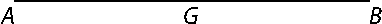
\includegraphics[width=0.40\textwidth]{gesamttex/edit_VIII,3/images/LH_35_09_15_018-019_d2.pdf}}%
  \vspace{0.5em}
  \centerline{\lbrack\textit{Fig.~2}\rbrack}%
%  \edtext{}{\lemma{\lbrack\textit{Fig.~2}\rbrack}\killnumber\Cfootnote{**************************}}
%  \newpage
  \vspace{1.5em}%
%
%
\count\Bfootins=900
\count\Afootins=1000
\count\Cfootins=900
\newpage
\pstart%
Duae chordae\protect\index{Sachverzeichnis}{chorda tensa}\edlabel{LH_35_09_15_018v_aliasdemonstrata_vldj-1}
ejusdem consistentiae,\protect\index{Sachverzeichnis}{consistentia chordae}
vel quod eadem edit\lbrack,\rbrack\
ejusdem chordae homogeneae\protect\index{Sachverzeichnis}{chorda homogenea}
duae partes diversae,
eam\edlabel{LH_35_09_15_018v_tensrupt-1}
tensionem qua rumpuntur\protect\index{Sachverzeichnis}{tensio rumpens}
habent eandem, sive
\edtext{cum rumpuntur
eodem modo sunt tensae.\edlabel{LH_35_09_15_018v_tensrupt-2}\protect\index{Sachverzeichnis}{chorda tensa}
Nam ruptura\protect\index{Sachverzeichnis}{ruptura chordae}
fit cum major est tensio\protect\index{Sachverzeichnis}{tensio chordae}}{%
\lemma{cum}\Bfootnote{%
\textit{(1)}~ita tensae sunt
\textit{(2)}~rumpuntur eodem modo sunt tensae
\textit{(a)}~, vel vires quibus rumpuntur
\textit{(b)}~. Chordae autem
\textit{(c)}~. Nam
\textit{(aa)}~tensio
\textit{(bb)}~ruptura
\textit{(aaa)}~in eo
\textit{(bbb)}~fit cum major est
\textit{(aaaa)}~vis tendens
\textit{(bbbb)}~tensio%
~\textit{L}}}
quam vis qua pars parti cohaeret;\protect\index{Sachverzeichnis}{vis cohaesionis}
quam vim ubique aequalem suppono. % [[vire]]
\edlabel{LH_35_09_15_018v_lexsimilitudinis-1}Ex generali autem lege\protect\index{Sachverzeichnis}{lex generalis}
similitudinum\protect\index{Sachverzeichnis}{lex similitudinum}
manifestum est,
duas chordas homogeneas\protect\index{Sachverzeichnis}{chorda homogenea}
sola longitudine\protect\index{Sachverzeichnis}{longitudo chordae} differentes
seu per omnia similes omnia habere proportionalia,\edlabel{LH_35_09_15_018v_lexsimilitudinis-2}
ac \edtext{proinde si vires tendentes\protect\index{Sachverzeichnis}{vis tendens}
sint ut longitudines,\protect\index{Sachverzeichnis}{longitudo chordae}
fore etiam tensiones\protect\index{Sachverzeichnis}{tensio chordae} aequales;
itaque vires quoque rumpentes\protect\index{Sachverzeichnis}{vis rumpens}
erunt ut longitudines,\protect\index{Sachverzeichnis}{longitudo chordae}
quia vires rumpentes\protect\index{Sachverzeichnis}{vis rumpens}
eandem faciunt tensionem\protect\index{Sachverzeichnis}{tensio chordae}}{%
\lemma{proinde}\Bfootnote{%
\textit{(1)}~tensiones
\textit{(2)}~vir
\textit{(3)}~si vires \lbrack...\rbrack\ etiam tensiones
\textit{(a)}~vel longitud
\textit{(b)}~aequales; itaque \lbrack...\rbrack\ ut longitudines,
\textit{(aa)}~quia vires proportionales longitudinibus eandem faciunt tensionem, 
\textit{(bb)}~et vires
\textit{(cc)}~quia vires \lbrack...\rbrack\ faciunt tensionem%
~\textit{L}}}
per
\edtext{paulo ante}{%
\lemma{paulo ante}\Cfootnote{%
S.~\refpassage{LH_35_09_15_018v_tensrupt-1}{LH_35_09_15_018v_tensrupt-2}}}
dicta; et
\edtext{vires\protect\index{Sachverzeichnis}{vis tendens} eandem facientes}{%
\lemma{vires}\Bfootnote{%
\hspace*{-0,5mm}eandem
\textit{(1)}~faciunt
\textit{(2)}~facientes%
~\textit{L}}}
tensionem\protect\index{Sachverzeichnis}{tensio chordae} sunt ut longitudines,
ergo vires rumpentes\protect\index{Sachverzeichnis}{vis rumpens}
duas chordas\protect\index{Sachverzeichnis}{chorda tensa} sola longitudine differentes,
sunt ut longitudines.\protect\index{Sachverzeichnis}{longitudo chordae}\edlabel{LH_35_09_15_018v_aliasdemonstrata_vldj-2}
\pend%
%
%
  \vspace{2.0em}%
%  \newpage
  \centerline{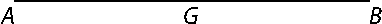
\includegraphics[width=0.40\textwidth]{gesamttex/edit_VIII,3/images/LH_35_09_15_018-019_d3.pdf}}%
  \vspace{0.5em}
  \centerline{\lbrack\textit{Fig.~3}\rbrack}%
%  \edtext{}{\lemma{\lbrack\textit{Fig.~3}\rbrack}\killnumber\Cfootnote{**************************}}
%  \newpage
  \vspace{1.5em}%
%
%
\count\Bfootins=1000
\count\Afootins=1000
\count\Cfootins=1000
\pstart%
Idem etiam ex eo demonstrabitur distinctius:
\edtext{dictum est,}{%
\lemma{dictum est}\Cfootnote{%
S.~\refpassage{LH_35_09_15_018r_aequtens-1}{LH_35_09_15_018r_aequtens-2}.}}
partes ejusdem chordae\protect\index{Sachverzeichnis}{chorda tensa} aequaliter tensas
in tensione\protect\index{Sachverzeichnis}{tensio chordae} illa
sustentari viribus\protect\index{Sachverzeichnis}{vis tendens}
quae sint ut longitudines,\protect\index{Sachverzeichnis}{longitudo chordae}
seu \textit{AG} dimidia vi in ea
\edtext{\lbrack tensione\rbrack}{%
\lemma{vi}\Bfootnote{\textit{L~ändert Hrsg.}}}
sustentari qua \textit{AB},
ergo et
\edtext{initio si duae separatae intelligantur \textit{AG} et \textit{AB},
viribus easdem \lbrack tensiones\rbrack\ accipient,}{%
\lemma{initio}\Bfootnote{%
\textit{(1)}~chorda \textit{AB}
\textit{(2)}~si duae \lbrack...\rbrack\ \textit{AG} et \textit{AB},
\textit{(a)}~eadem
\textit{(b)}~viribus
\textit{(aa)}~tende
\textit{(bb)}~easdem \textbar~tensionem \textit{ändert Hrsg.}~\textbar\ accipient,%
~\textit{L}}}
quae sint ut chordae \textit{AG} et \textit{AB},
cum tensionem nactae sunt.
Verum duae
\edtext{chordae\protect\index{Sachverzeichnis}{chorda tensa}
ejusdem consistentiae\protect\index{Sachverzeichnis}{consistentia chordae}
in iisdem tensionibus,\protect\index{Sachverzeichnis}{tensio chordae}
habent viribus tendentibus\protect\index{Sachverzeichnis}{vis tendens}
proportionales longitudinum\protect\index{Sachverzeichnis}{longitudo chordae}}{%
\lemma{chordae}\Bfootnote{%
\textit{(1)}~$\langle$\textendash$\rangle$ et pr
\textit{(2)}~eande
\textit{(3)}~ejusdem consistentiae
\textit{(a)}~eandem tensionem
\textit{(b)}~in iisdem tensionibus, habent
\textit{(aa)}~tensiones suas
\textit{(bb)}~longitudi
\textit{(cc)}~viribus tendentibus proportionales longitudinum%
~\textit{L}}}
differentias
%
\lbrack19~r\textsuperscript{o}\rbrack\ % % % % Blatt 19r
%
seu acquisitiones longitudinum\protect\index{Sachverzeichnis}{longitudo chordae acquisita}
viribus proportionales;
ergo et longitudinibus % [[quo]]
integris quaesitis,\protect\index{Sachverzeichnis}{longitudo chordae quaesita}
ergo et longitudinibus initialibus.\protect\index{Sachverzeichnis}{longitudo chordae initialis}
Ergo vires eodem modo tendentes\protect\index{Sachverzeichnis}{vis tendens}
erunt chordarum longitudinibus ante tensionem
seu naturalibus\protect\index{Sachverzeichnis}{chordae longitudo naturalis} proportionales.
Si
\edtext{priore principio}{\lemma{priore principio}\Cfootnote{%
Siehe S.~\refpassage{LH_35_09_15_018v_lexsimilitudinis-1}{LH_35_09_15_018v_lexsimilitudinis-2}.}}
%
utamur,
sumto a similitudine omnium,\protect\index{Sachverzeichnis}{principium a similitudine omnium}
hinc poterimus demonstrare quaedam in
posteriori demonstratione\protect\index{Sachverzeichnis}{demonstratio}
assumta.
\pend%
%
\newpage
  \centerline{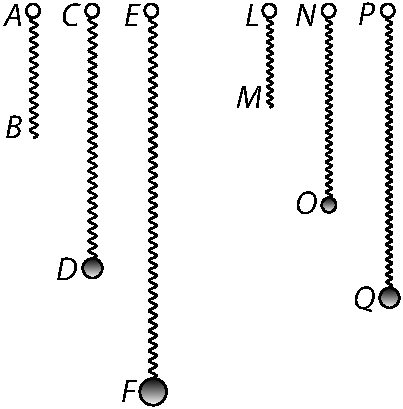
\includegraphics[width=0.33\textwidth]{gesamttex/edit_VIII,3/images/LH_35_09_15_018-019_d4.pdf}}%
  \vspace{0.5em}
  \centerline{\lbrack\textit{Fig.~4}\rbrack}%
  \vspace{1.5em}%
\pstart%
Ex natura similitudinis\protect\index{Sachverzeichnis}{natura similitudinis} debet \edlabel{LH_35_09_15_019r_marginalie_zdotiu-1}%
esse%
\edtext{}{%
\lemma{\textit{Nach} esse \textit{über der Zeile:}}\Afootnote{\astrosun\vspace{-4mm}}}%
\edlabel{LH_35_09_15_019r_marginalie_zdotiu-2}
 % [[\textit{AB}]]
%%
$\displaystyle\overline{CD : EF},\, : \overline{D : F} \squaredots \overline{NO : PQ},\, : \overline{O : Q}.$
Id est erunt proportionalitates\protect\index{Sachverzeichnis}{proportionalitas} saltem\lbrack,\rbrack\
seu proportionum proportiones\protect\index{Sachverzeichnis}{proportio proportionum}\lbrack,\rbrack\
inter se aequales.
Ergo siquando erunt \textit{D} ad \textit{F} ut \textit{O} ad \textit{Q},
illo casu erunt $\displaystyle CD : EF \,\squaredots\, NO : PQ,$
vel contra si esset \textit{F} dupla \textit{D}, et \textit{Q} tripla \textit{O},
fieret $\displaystyle2\, CD : EF \,\squaredots\, 3\, NO :
\edtext{PQ.$
Demonstratum est
\edtext{\edlabel{LH_35_09_15_019r_alibi_iocslg-1}alibi\edlabel{LH_35_09_15_019r_alibi_iocslg-2}}{%
\lemma{alibi}\Cfootnote{%
Siehe hierüber die Erläuterung zu S.~\refpassage{LH_35_09_15_018r_alias_sjhvbis-1}{LH_35_09_15_018r_alias_sjhvbis-2}.}}
fore}{%
\lemma{\textit{PQ.}}\Bfootnote{%
\textit{(1)}~Ponamus esse
\textit{(2)}~Demonstratum est alibi fore%
~\textit{L}}}
$\displaystyle \overline{CD - AB} : \overline{EF - AB} \,\squaredots\, D : F,$
ergo similiter
$\displaystyle\overline{NO - LM},\, : \overline{PQ - LM} \,\squaredots\, \edtext{O : Q.$
Quibus duobus valoribus\protect\index{Sachverzeichnis}{valor} tollentur
\textit{D} \!:\! \textit{F} et \textit{O} \!:\! \textit{Q},
ex priori eritque:}{%
\lemma{$O : Q.$}\Bfootnote{%
\textit{(1)}~Quae jungendo prioribus f
\textit{(2)}~Quibus duobus \lbrack...\rbrack\ priori eritque:%
~\textit{L}}}
$\displaystyle \overline{CD : EF} : \overline{\overline{CD - AB} : \overline{EF - AB}} \,\squaredots\, \overline{NO : PQ} : \overline{\overline{NO - LM} : \overline{PQ - LM}}.$
Seu
$\displaystyle \overline{CD : EF} : \overline{NO : PQ}$
rationes linearum,\protect\index{Sachverzeichnis}{linea tensa}
sunt ut
$\displaystyle \squaredots\ \overline{\overline{CD - AB} : \overline{EF - AB}} :
\overline{\overline{NO - LM} : \overline{PQ - LM}}$
% \edtext{}{\lemma{$\displaystyle \squaredots\ \overline{\overline{CD - AB} : \overline{EF - AB}} : \overline{\overline{NO - LM} : \overline{PQ - LM}}$}\Bfootnote{\textit{erg.~L}}}
rationes differentiarum cujusque
\edtext{in statu naturali.%
\protect\index{Sachverzeichnis}{status chordae}\protect\index{Sachverzeichnis}{status naturalis}}{%
\lemma{in}\Bfootnote{%
\textit{(1)}~linea
\textit{(2)}~statu naturali.%
~\textit{L}}}
\pend
%
\pstart%
Hinc siquando $\displaystyle CD : EF \,\squaredots\, NO : PQ,$
erit etiam $\displaystyle \overline{CD - AB} : \overline{EF - AB} \,\squaredots\, \overline{NO - LM} : \overline {PQ - LM}.$
Est autem $\displaystyle CD\cdot PQ$ aequ. $\displaystyle EF\cdot NO,$
fiet:
\pend
\vspace{0.21mm}
\pstart
\noindent
\ovalbox{$\displaystyle\overset{\displaystyle CD\cdot PQ}{EF\cdot NO}$}
$\displaystyle\overset{\displaystyle \!-\, CD\cdot LM - AB\cdot PQ}{\!-\, EF\cdot LM - AB\cdot NO}$
\ovalbox{$\displaystyle\overset{\displaystyle \!+\, AB\cdot LM}{\!+\, AB\cdot LM.}$}
\!$\displaystyle\overset{\displaystyle\text{aequ.}}{\phantom{XXX}}$
%%%%%%%%% NB: Die folgenden zwei Druckzeilen müssen zusammenbleiben !!!!!!!!!!!!!!
% \newline% (Zeile 1)
% $\displaystyle CD.\, PQ \,-\, CD.\, LM \,-\, AB.\, PQ \,+\, AB.\, LM$ aequ.
% \newline% (Zeile 2)
% $\displaystyle EF.\, NO \,-\, EF.\, LM \,-\, AB.\, NO \,+\, AB.\, LM.$
%%%%%%%%% NB: Die vorherigen zwei Druckzeilen müssen zusammenbleiben !!!!!!!!!!!!!!
\pend
%
\vspace{0.3mm}
\pstart%
Ergo $\displaystyle \overline{EF - CD} : AB \,\squaredots\, \overline{PQ - NO} : LM.$
% \pend
%
% \pstart%
Et quia \textit{CD} potest poni \textit{vEF},
et eodem modo \textit{NO} poni potest \textit{vPQ},
fiet:
$\displaystyle \overline{EF - vEF} : AB \,\squaredots\, \overline{PQ - vPQ} : LM,$
et divisis omnibus per $1 - v,$
fiet
$\displaystyle EF : AB \,\squaredots\, PQ : LM.$
\pend
\newpage
 %
\pstart%
Ergo si pondera tendentia\protect\index{Sachverzeichnis}{pondus tendens}
sint \edtext{proportionalia\lbrack,\rbrack\
etiam lineae tensae\protect\index{Sachverzeichnis}{linea tensa}
eandem servabuntur proportionem}{%
\lemma{proportionalia}\Bfootnote{%
\textit{(1)}~erunt
\textit{(2)}~etiam lineae \lbrack...\rbrack\ servabuntur proportionem%
~\textit{L}}}
ad primam;
et vicissim sequetur
lineis\protect\index{Sachverzeichnis}{linea tensa} proportionaliter crescentibus
pondera\protect\index{Sachverzeichnis}{pondus tendens} quoque proportionaliter crescere
\edtext{debere.
Seu si \textit{F} ad \textit{D} ut \textit{Q} ad \textit{O},
erit quoque
\textit{EF}, \textit{CD}, \textit{AB} $\displaystyle\squaredots$ \textit{PQ}, \textit{NO}, \textit{LM}.}{%
\lemma{debere.}\Bfootnote{%
\textit{(1)}~Sed
\textit{(a)}~pondu
\textit{(b)}~demonstratum est fore $CD : E$
\textit{(2)}~Seu si \lbrack...\rbrack\ erit quoque
\textit{(a)}~\textit{EF} ad \textit{AB}, ut \textit{PQ} ad \textit{LM}
\textit{(b)}~\textit{EF}, \textit{CD}, \textit{AB} $\displaystyle\squaredots$ \textit{PQ}, \textit{NO}, \textit{LM}.%
~\textit{L}}}
% \pend
%
% \pstart%
Et
\edtext{vicissim.
Sed haec}{%
\lemma{vicissim.}\Bfootnote{%
\textit{(1)}~Si sint
\textit{(2)}~Sed haec%
~\textit{L}}}
jam satis patent ex prima analogia\protect\index{Sachverzeichnis}{analogia}
\edtext{sub signo\protect\index{Sachverzeichnis}{signum} \astrosun.}{%
\lemma{sub signo \astrosun}\Cfootnote{%
Siehe die Randbemerkung zu S.~\refpassage{LH_35_09_15_019r_marginalie_zdotiu-1}{LH_35_09_15_019r_marginalie_zdotiu-2}.}}
\pend%
%
%
%
%  \newpage
 %  \edtext{}{\lemma{\lbrack\textit{Fig.~4}\rbrack}\killnumber\Cfootnote{**************************}}
%  \newpage
%  \vspace*{2.0em}%
%
%
%
% ENDE DES STÜCKES auf Blatt 19r
\count\Bfootins=1200
\count\Afootins=1200
\count\Cfootins=1200